% !TeX spellcheck = cs_CZ
\wikitextrule
\begin{example}\label{FYZ:exam006}
  Najděte paralaxu Proximy Centauri, která je od nás vzdálená asi \num{4.2} světelného roku 
  \protect\cite[s.~4]{Kulhanek2009}.
  
   {\centering
    \captionsetup{type=figure}
    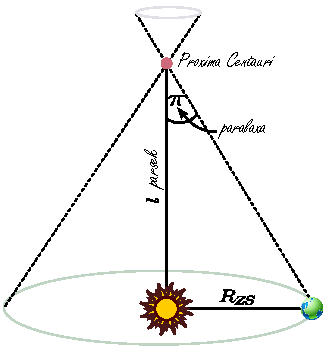
\includegraphics[width=0.8\linewidth]{fyz_fig225.pdf}
    \captionof{figure}{K příkladu \ref{FYZ:exam006}: Paralaxa naší nejbližší hvězdy}
    \label{fyz:fig225}
    \par}
    
  \textbf{Řešení}: Díky pohybu Země kolem Slunce se zdá, že blízké hvězdy opisují oproti 
  vzdáleným elipsu. Úhlový poloměr této elipsy se nazývá paralaxa hvězdy. Lze ji změřit jen pro 
  nejbližší hvězdy. Z definice úhlu (jako v předchozím příkladě) tedy vyplývá, že
  \begin{equation*}
    \pi = \frac{R_{ZS}}{l} = \frac{\SI{1.5e11}{\meter}}{\SI{4.2}{\lightyear}} 
        = \frac{\SI{1.5e11}{\meter}}{\num{4,2}\cdot\SI{9.5e15}{\meter}}
          \cong \SI{3,7e-6}{\radian},
  \end{equation*}
  
  což je přibližně \(\ang{;;0,76}\). Vidíme, že i u druhé nejbližší hvězdy po Slunci není 
  paralaxa ani celá \(\ang{;;1}\).
\end{example}
\wikitextrule